\subsection{Mécaniques de jeu}

	\subsubsection{Cahier des charges}

		\paragraph{Objectif du jeu}
			Chaque joueur se voit attribuer une cible et est lui-même la cible d'un autre joueur.
			Nous intégrerons donc un système de sélection de cibles, et un moyen pour le joueur de sélectionner un personnage (joueur ou non) à proximité de lui.
			
			Le but est de tuer le plus de joueurs cibles dans le temps imparti.
			Chaque assassinat rapporte X points aux joueurs.
			
			À l'aide de classes de personnage, nos personnages \textbf{pourraient} avoir des pouvoirs spécifiques,
			tel que se déguiser en quelqu'un d'autre pendant une durée limitée,
			pouvoir tuer à moyenne distance, ralentir et affaiblir un joueur
			(l'empêcher de courir, d'utiliser des capacités par exemple), avoir une boussole plus précise\dots
			
			
			Nous avons également rajouté des objets pouvant être utilisés par les joueurs
			(Echelles\footnote{Voir Figure 4}, Portes) et comptons en rajouter d'autres.
			\begin{figure}[hbt!]
				\centering
				\begin{subfigure}[t]{0.3\textwidth}
					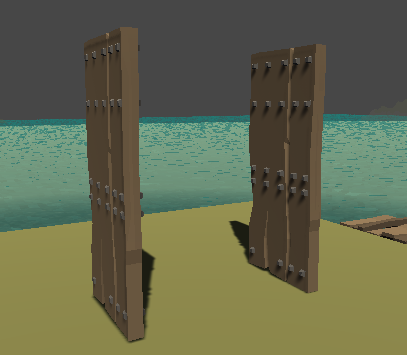
\includegraphics[scale=0.41]{doors_open.png} 
					\caption{Portes ouvertes}
				\end{subfigure}
				\hspace{50pt}
				\begin{subfigure}[t]{0.3\textwidth}
					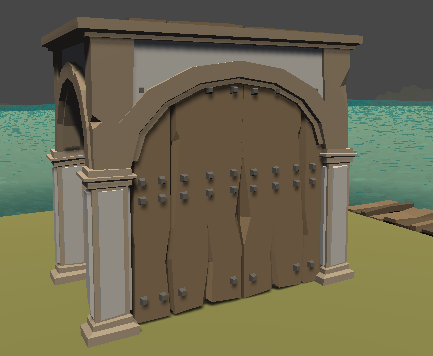
\includegraphics[scale=0.39]{doors_closed.png}
					\caption{Porte fermée avec arche}
				\end{subfigure}
				\caption{Exemple des portes que nous avons réalisé}
			\end{figure}
			\FloatBarrier

		\paragraph{Organisation de partie}
			L'organisation de partie concerne la création des scripts et ressources permettant à 
			chaque partie multijoueur de se dérouler suivant un schéma prédéterminé. Cela comprend le début et 
			la fin de manche (choix du gagnant, présentation du classement de fin de partie par exemple), le placement des éléments 
			dynamiques de la scène, les timers, le comptage des points, l'assignation des cibles...

			Pour offrir la meilleure expérience de jeu possible, cette organisation doit permettre à chaque manche d'être unique et imprévisible.
			Pour cela, nous introduirons de la complexité dans les différentes mécaniques de jeu. Par exemple, on peut attribuer plus de points
			au premier joueur ayant abattu sa cible ou à un joueur ayant survécu un certain temps sans se faire tuer.


			
	\subsubsection{Première soutenance}

        \paragraph{Environnement}

            Nous nous sommes beaucoup inspirés du mode multijoueur des premiers Assassin's Creed. Le système de grimpe s'étant 
			montré trop complexe à mettre en place, nous avons réutilisé quelques idées de gameplay pour l'environement, comme les échelles et les portes.

            \begin{figure}[hbt!]
                \centering
                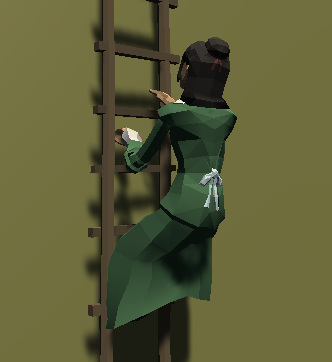
\includegraphics{ladder.png}
                \caption{Joueur grimpant sur l'échelle}
            \end{figure}
			\FloatBarrier

            Les échelles permettent de créer un peu de verticalité dans nos niveaux.
            Elles ne peuvent être utilisées que par les joueurs, mais ont leurs avantages comme leurs inconvénients : ainsi,
            prendre de la hauteur permet d'emprunter des raccourcis, mais retire la discrétion (car personne de civilisé devrait être sur les toits !)
            
            Les portes permettent de barrer le passage pour échapper à son agresseur.
            Elles se ferment quand le joueur passe dessus en courant
            et se rouvrent au bout de quelques secondes.

            \begin{figure}[ht]
                \centering
                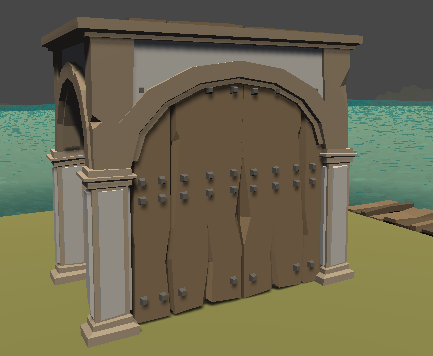
\includegraphics{doors_closed.png}
                \caption{Porte fermée après le passage d'un joueur}
            \end{figure}
			\FloatBarrier


        \paragraph{Déplacement du personnage}
            
            Tout jeu est très rapidement limité par la capacité de déplacement du personnage et sa vitesse.
            Nous avons donc réalisé un script de déplacement qui permet au joueur de marcher, courir, sauter et grimper aux échelles.

            Pour le côté technique, nous avons dans un premier temps utilisé l'Input System de base proposé par Unity. Mais plusieurs problèmes se sont posés:
            \begin{itemize}
                \item Les configurations des keymaps sont assez limitées
                \item Paramétrer des périphériques autre que le clavier/souris est compliqué. Il faudrait avoir des scripts différents pour chaque périphérique, et donc des prefabs différents
            \end{itemize}
            C'est pour cette raison que nous avons migré vers le New Input System.
            Celui ci est ergonomique, multiplateforme et permet l'utilisation de périphériques divers, comme la manette ou le clavier par exemple.
            Certains scripts ont dû être modifiés pour devenir compatibles avec ce système.

            Il est donc actuellement possible de jouer au clavier/souris ou à la manette (pas les deux à fois).
            
        \paragraph{Attribution des cibles}
            
            Harrys a réalisé le script permettant l'attribution des cibles, qui utilise des méthodes RPC (communication inter-clients par l'intermédiaire d'un serveur). Le "MasterClient", un client qui est désigné dans chaque salle pour faire office de maître de jeu, est celui qui séléctionne la cible de chaque joueur. Il communique ensuite à chacun des clients présents dans la salle sa cible désignée. Cette attribution se fait de façon aléatoire, mais selon certaines règles:
            \begin{itemize}
                \item Un joueur ne peut (évidemment) pas être sa propre cible
                \item Deux joueurs ne peuvent pas être la cible l'un de l'autre (Cela permet une plus grande interaction entre les joueurs et pas simplement des scénarios en "1 contre 1").
                \item Plusieurs joueurs ne peuvent pas avoir la même cible.
            \end{itemize}
                
            Cependant même si ce script est fonctionnel, il n'a pas encore été implémenté. 
            Le système d'élimination de la cible fera l'objet d'un travail important pour la prochaine soutenance.
        
        
        \paragraph{Système de verrouillage}
            
            Le système qui attribue des cibles à chaque joueur n'est pas entièrement implémenté, mais le joueur peut déjà tuer une cible, qu'elle soit la bonne ou non.
            Pour cela, il passe en mode verrouilage, et les personnages pointés par le viseur surbrillent.
            Pour les sélectionner, un coup de molette suffit, et le contour devient alors jaune, pour indiquer que la cible est verouillée.
            Il suffit alors d'être à moins d'un mètre pour l'éliminer\footnote{Voir fig 6}.

            \begin{figure}[hbt!]
                \centering
                \begin{subfigure}[b]{0.3\textwidth}
                    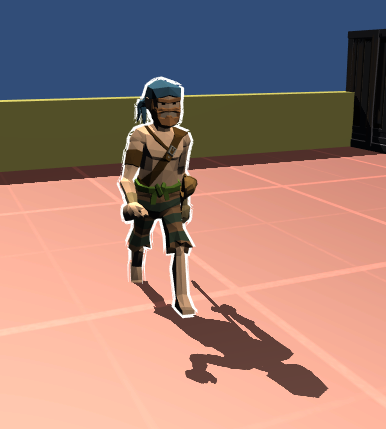
\includegraphics[scale=0.44]{white_outline.png} 
                    \caption{Personnage en surbrillance}
                \end{subfigure}
                \hspace{150pt}
                \begin{subfigure}[b]{0.3\textwidth}
                    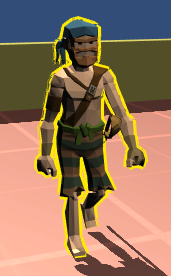
\includegraphics[scale=0.8]{yellow_outline.png} 
                    \caption{Personnage sélectionné et verrouilé}
                \end{subfigure}

                \begin{subfigure}[b]{0.3\textwidth}
                    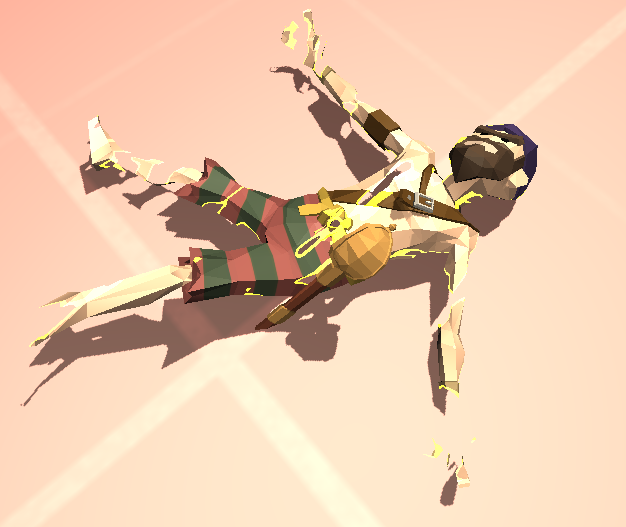
\includegraphics[scale=0.27]{death.png} 
                    \caption{Disparition des corps après mort}
                \end{subfigure}
                \caption{Système de verrouilage}
            \end{figure}
			\FloatBarrier

            Pour le material qui fait disparaître les corps, nous avons créé manuellement un shader avec l'outil Shader Graph de Unity\footnote{Voir fig 7}.
            Nous pouvons donc créer des shaders personnalisés et dynamiques (avec comme exemple l'utilisation du temps).

            \begin{figure}[hbt!]
                \centering
                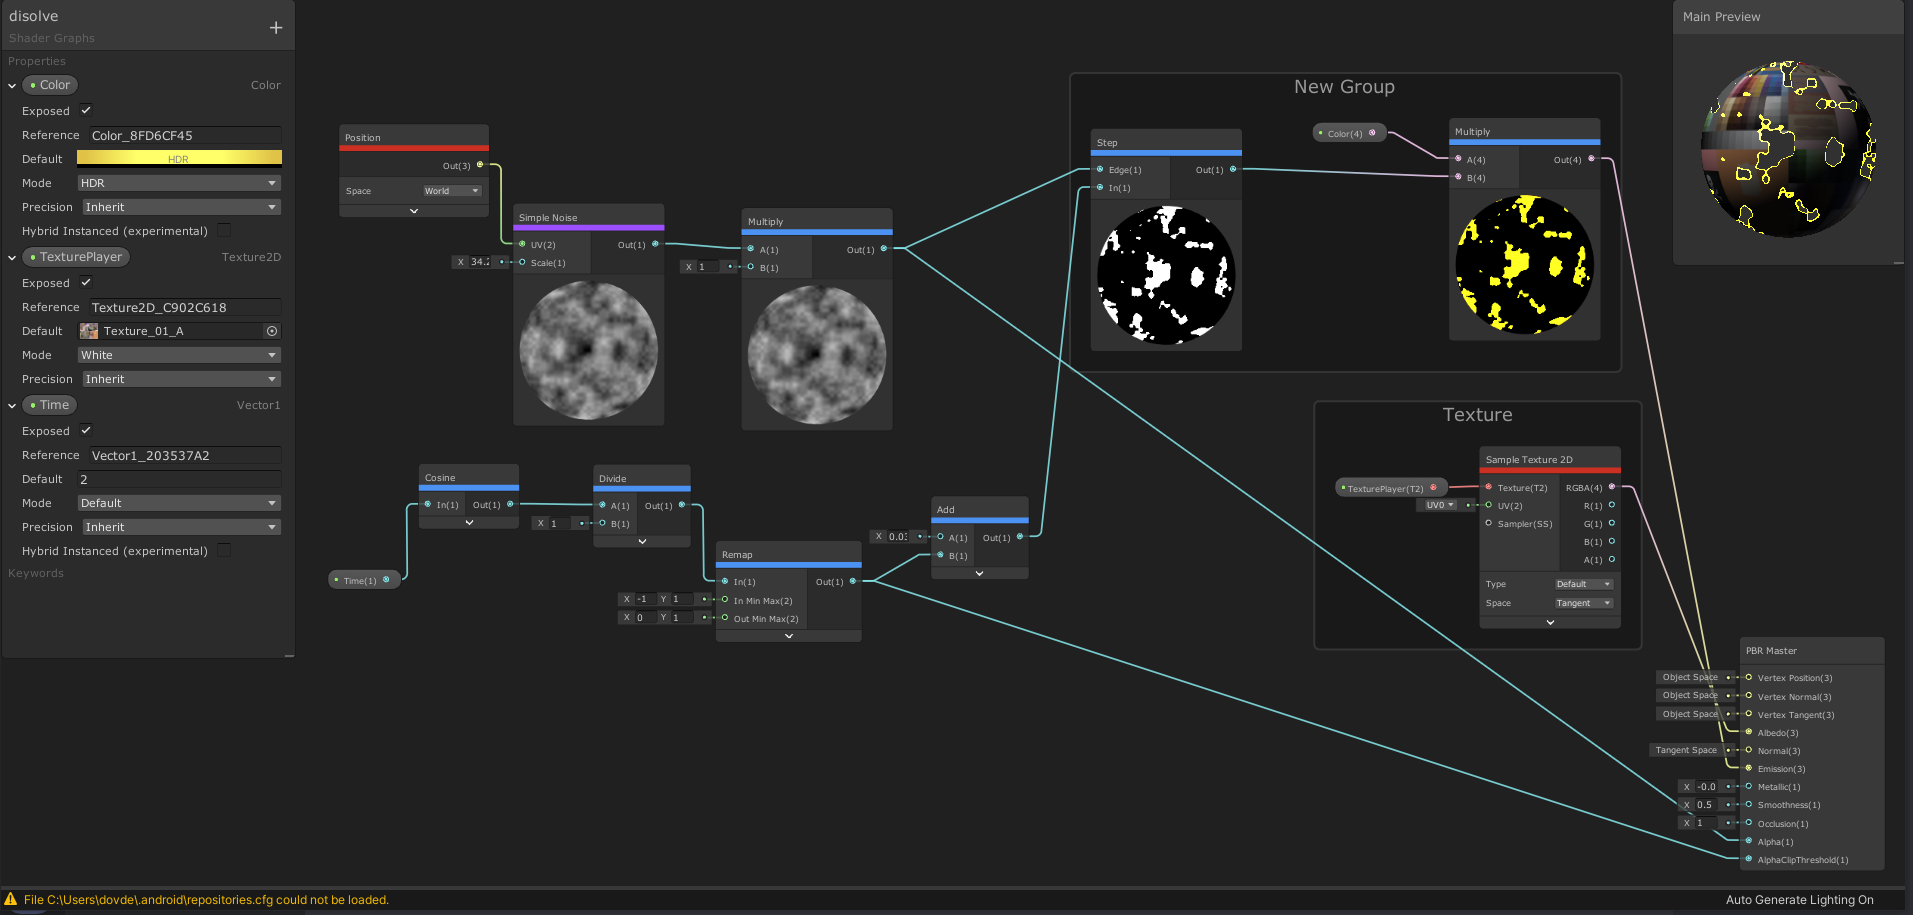
\includegraphics[scale=0.29]{dissolve_shader.png}
                \caption{Vue du shader créé depuis Shader Graph}
            \end{figure}
			\FloatBarrier



	\subsubsection{Deuxième soutenance}

		\paragraph{Système de verrouillage}

			Pour tuer un personnage (joueur ou NPC),
			nous avons ajouté un système de verrouillage. Celui-ci est assez pratique : lorsque l'on passe dans ce mode, l'écran change et 
			un effet réalisé grâce au post processing de Unity permet de donner un effet sépia/vieux films\footnote{voir Effets Graphiques}.
			Un contour blanc autour des personnages visés au centre de l'écran permettent voir quel personnage va être sélectionné.

			Une fois sa cible sélectionnée, le joueur peut l'éliminer à condition d'en être suffisamment proche.

			L'effet a demandé de créer plusieurs overlays de caméra, afin d'avoir un effet graphique
			appliqué uniquement sur certains layers, et de les surperposer les uns sur les autres. 

		\paragraph{Finishers}
			Nous avons fourni un vrai travail sur les différentes animations de mort des personnages.
			Lors de sa réalisation, un problème s'est posé : Il fallait que les animations de deux GameObject (ici le joueur qui tue et le NPC/joueur tué) 
			soient parfaitement synchronisées. Après avoir regardé plusieurs types de solutions, nous nous sommes tournés vers un outil préintégré appelé Timeline.
			Ce dernier permet de réaliser des clips vidéos.

			Voici donc comment nous avons intégré les timelines :
			
			Des faux personnages jouant les animations sont ajoutés sur la carte à la position et rotation du tueur.
			On masque le tueur et la victime de la carte.
			On change le mesh et le matériau de chaque personnage de la timeline pour qu'il corresponde au tueur et au
			personnage tué.

			Une fois l'animation terminée, un signal est envoyé à un script qui réaffiche alors le joueur qui était masqué.
			Si le personnage tué était un joueur, alors il réapparait discrètement ailleurs sur la map lors de sa réaparition.
			Le personnage tué disparait de la carte au bout d'une dizaine de secondes avec un shader fait avec Shader Graph.

			Voici quelques finishers que nous avons réalisé :

			\begin{figure}[hbt!]
				\centering
				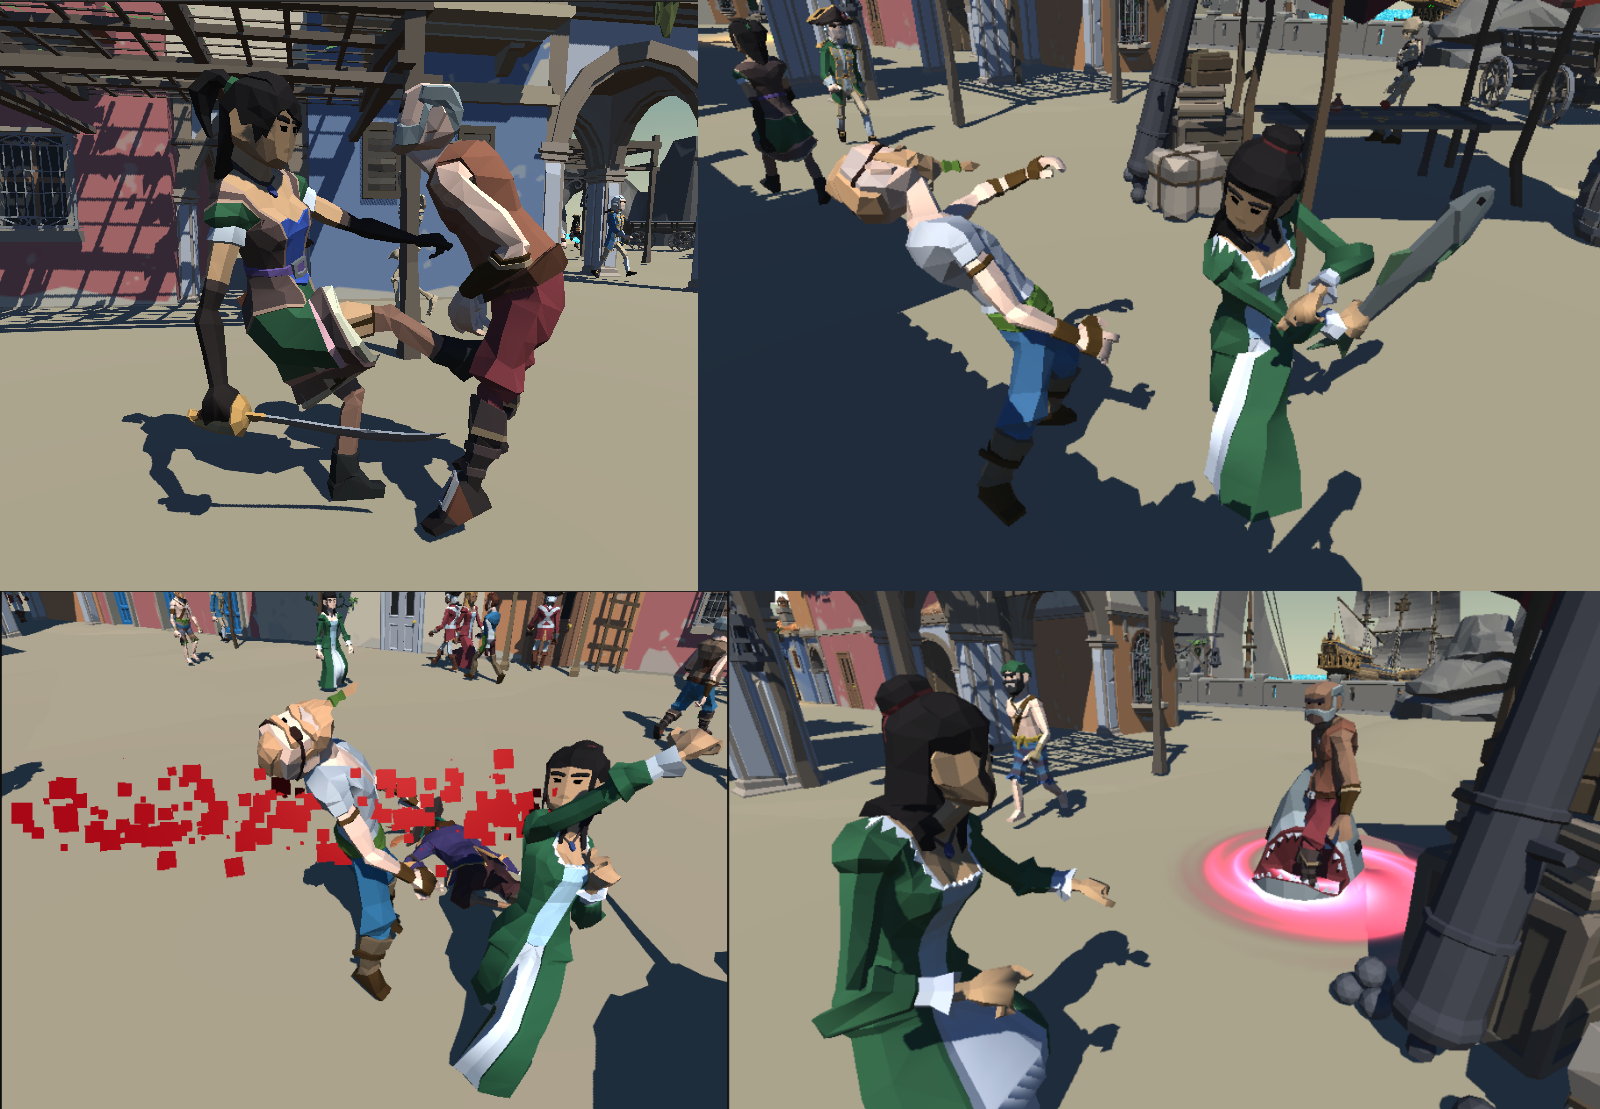
\includegraphics[scale=0.25]{finishers/finishers.png}
				\caption{Quelques finishers}
			\end{figure}

			\FloatBarrier
			\begin{figure}[hbt!]
				\centering
				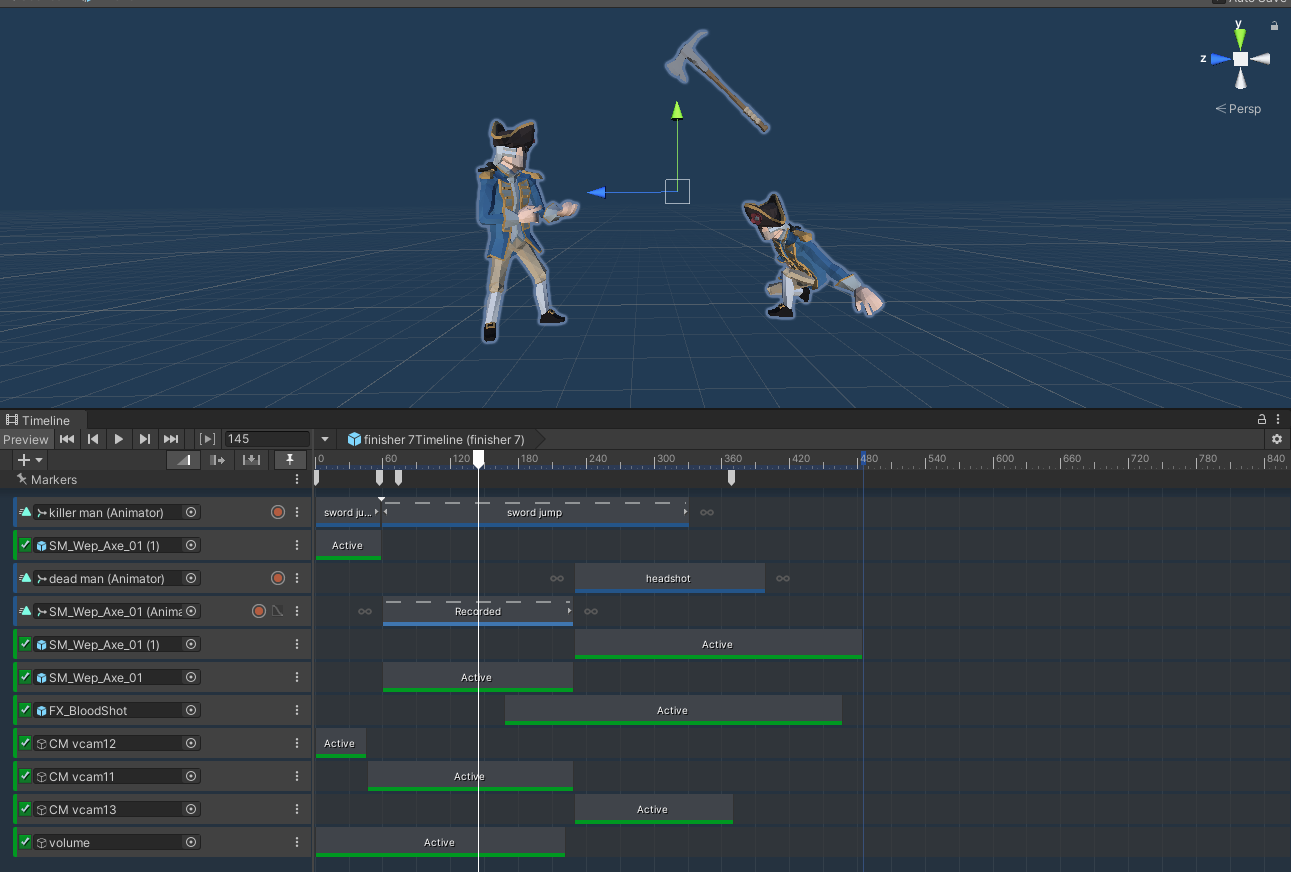
\includegraphics[scale=0.3]{timeline_hache.png}
				\caption{Timeline du lancer de hache}
			\end{figure}
			\FloatBarrier


		\paragraph{Système de manche}

			Le système actuellement utilisé pour le déroulement d'une partie se base sur des manches. Le jeu se fait en deux phases:
			\begin{itemize}
				\item Une période de 'grâce' de 30 secondes où les joueurs attendent l'assignation d'une cible. Ils sont libres de se déplacer, pour se cacher par exemple.
				\item Une période de 'chasse'. Les cibles sont assignées et le combat peut commencer. Elle est au départ de 3 minutes, mais ce temps
				diminue à chaque mort de joueur pour pousser les participants au meurtre.
			\end{itemize}
		

		\paragraph{Système de mort}

			Joueurs comme IA peuvent être tués. Dans le cas d'un joueur, un système de mort a été mis en place. Ainsi,
			quand le joueur se fait tuer, son personnage est désactivé temporairement et il rentre
			en mode "spectateur". Il peut se balader sur la map, mais il ne peut en aucun cas interagir avec l'environnement,
			et il n'est pas visible des autres joueurs. Une fois la manche terminé, le joueur réapparait aléatoirement sur la map.


		\paragraph{Système de point}

			Un système de point a également été implémenté. Il fonctionne de la façon suivante:
				-Tuer sa cible rapporte des points. le premier joueur tuant sa cible gagne plus de point, les autres en gagne de moins en moins.
				-Tuer une IA fait perdre des point! Il faut donc faire attention à ne pas tuer n'importe qui. Celà encourage la réflexion et pas simplement un carnage afin de trouver sa cible.
				-Tuer la cible de quelqu'un d'autre ne fait pas perdre de points, mais un système de compensation a été mis en place. Ainsi, se faire voler sa cible par un autre joueur apporte des points de compensation. Encore une fois, il n'est donc pas dans l'intérêt 
				des joueurs de tuer le premier venu
				-Une autre façon de gagner des points et d'être encore en vie à la fin d'une manche.
			Tous ces éléments permettent de déterminer le classement de la partie.
	

		\paragraph{Système de fin de partie}

			Finir une partie est tout un processus. Il faut d'abord désactiver le mouvement des joueurs.
			On présente ensuite plusieurs informations comme le rang final, le nombre d'assassinats
			et de mort, ainsi que l'expérience acquise. Il y a également une sauvegarde de ses statistiques et une mise à jour du système
			de niveau dans le but de permettre leur utilisation éventuel par le système de progression.
			Ensuite, on propose au joueur de rejouer. S'il refuse, il quitte la salle et peut fermer le jeu ou rejoindre une autre salle.
			Sinon, quand tout les joueurs ont décidé de redémarrer ou de partir, les joueurs retournent 
			sur le lobby dans l'attente d'une nouvelle partie.


		\paragraph{Cinemachine}

			Cinemachine est un suite modulaire d'outils de caméras pour Unity, qui offre 
			une qualité de contrôle de la caméra digne de jeux AAA. Cinemachine est conçu pour être utilisé 
			avec toutes les caméras d'un projet, mais peut aussi être utilisé en parallèle des caméras existantes. 
			Les Dolly track (rails de caméras) permettent de créer des animations de début de jeu ou 
			des vidéos de présentation beaucoup plus facilement qu'avec le système de caméras intégrées. 

			A l'échelle du jeu, Cinemachine est utilisé sur la quasi-totalité des caméras, 
			afin de permettre une transition douce entre la première et la troisième personne et pour 
			proposer des cinématiques plus vivantes, avec des déplacements et des focus.



	\subsubsection{Dernière soutenance}

		\paragraph{Correction de bugs}
			
			Lors de cette dernière période, nous avons cherché et supprimé certains bugs qui avaient notamment lieu au niveau des objets comme les échelles ou les bancs. 
			Certains étaient liés à des erreurs de code, et d'autres à une utilisation de certains objets à des endroits inadaptés.
			Les échelles ont été améliorées, ainsi que les lumières (qui recontraient de gros problèmes) et le système de 
			sélection, dont le fonctionnement était un peu aléatoire.

		\paragraph{Ajout des tyroliennes}

			Cependant, il nous manquait un élément présent dans beaucoup de jeux: une tyrolienne, permettant de laisser la 
			gravité faire son travail pour se déplacer d'un point à un autre. Nous avons donc rajouté un asset permettant 
			de créer des cordes, et avons créé un objet tyrolienne comprenant tous les prefabs et scripts nécéssaires.

			\begin{figure}[hbt!]
				\centering
				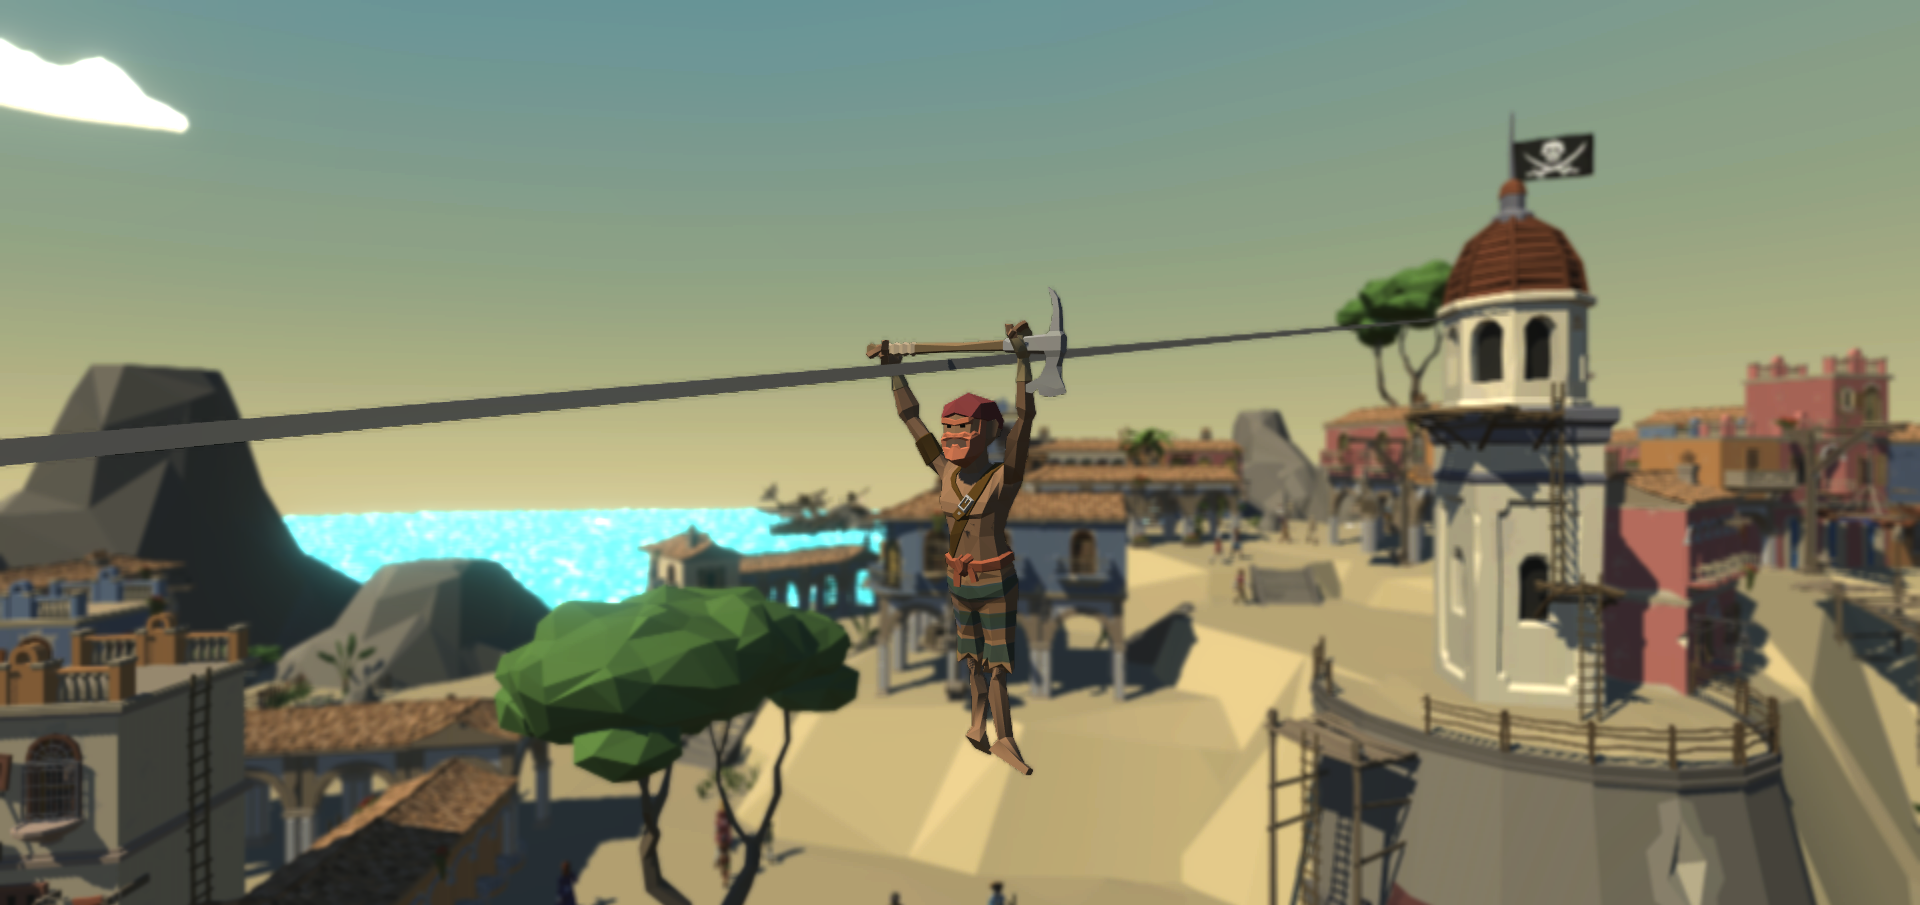
\includegraphics[scale=0.22]{zipline.png}
				\caption{Vue de la tyrolienne de l'île de Tortuga}
			\end{figure}
			\FloatBarrier

			Ces dernières téléportent le joueur au point de départ, désactivent 
			sa gravité et son contrôleur, puis lui appliquent des transformations 
			successives dans la direction du point d'arrivée. Il est également possible 
			de s'en extraire en sautant, ce qui provoque une chute suivie d'une animation 
			d'amortie à l'arrivée.

		\paragraph{Déguisement}

			Le mode déguisement est un pouvoir qui permet au joueur de prendre pendant une dizaine de secondes l'apparence 
			d'un personnage (joueur ou non) à proximité. Ce pouvoir permet de fuir son agresseur, et se montre très pratique 
			en particulier lorsque ce dernier vous a aperçu et est trop proche de vous pour avoir accès à la boussole. 
			Le jeu caste aux alentours les personnages, et retourne l'apparence (matériau/texture + mesh) du 
			personnage le plus proche s'il existe, et d'un personnage au hasard sinon.

		\paragraph{Pouvoirs}

			La nouveauté majeure de cette troisième soutenance est la possibilité d'utiliser des pouvoirs, actuellement au 
			nombre de quatre, afin de choisir un avantage majeur au cours de la partie. Les pouvoirs permettent de diversifier 
			le jeu et de proposer une expérience de jeux adaptée à tous en fonction de leurs compétences.

		\paragraph{Bombe de fumée}

			La bombe de fumée est, comme son nom tend à l'indiquer, un objet qui active des particules autour d'un joueur lui 
			permettant de créer une confusion afin de se retirer ou d'attaquer discrètement. Son grand intérêt réside dans le fait 
			qu'elle paralyse tous les personnages, NPC comme joueurs (sauf le lanceur, bien évidemment) jusqu'à dissipation de la fumée. 
			C'est donc un atout majeur de fuite plus que d'attaque.

		\paragraph{Poison}

			Le poison n'est pas vraiment un atout en jeu, car il nécéssite de suivre sa victime et de la tuer comme pour une 
			élimination classique. Cependant, lors de l'élimination de la cible, cette dernière donne plus de points, car son 
			élimination est discrète.
			
			\begin{figure}[hbt!]
				\centering
				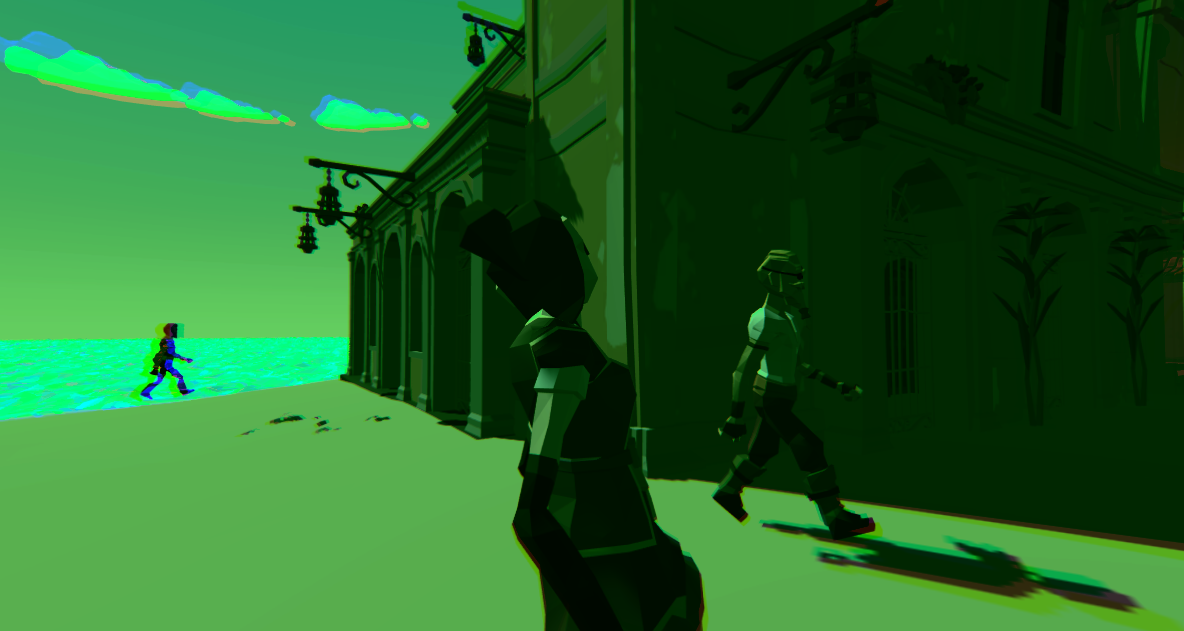
\includegraphics[scale=0.35]{poison.png}
				\caption{Agonie d'un personnage empoisonné}
			\end{figure}
			\FloatBarrier

		
		\paragraph{Lancer de couteaux}

			Le pouvoir du lancer de couteaux est de loin celui ayant été le plus long à mettre en oeuvre. Lorsque l'assassin 
			verrouille sa cible, il peut lui lancer un couteau jusqu'à 15 mètres (contre 2 mètres pour les attaques classiques).
			La cible touchée se met à boiter, voit sa vitesse réduite et ne peut ni courir, ni emprunter d'échelles pendant une certaine 
			période donnant à son assaillant le temps de l'achever. D'un point de vue technique, une refonte totale des animations *
			a eu lieu, afin que les personnages boiteux aient une animation spécifique. De nombreux nouveaux cas pour la course, les 
			échelles et les tyroliennes ont également dû être gérés. 


		\paragraph{Sprint}
	
			Le pouvoir de sprint permet au joueur de se déplacer très rapidement et d'être invulnérable face aux attaques 
			au couteau. En revanche, le joueur ne peut pas emprunter d'échelles ou de tyroliennes en même temps que ce pouvoir, afin 
			de ne pas déséquilibrer le jeu. Il laisse également une longue traînée de fumée derrière lui, qui lui fait perdre 
			tout semblant de discrétion. D'un point de vue technique, l'attribut vitesse du joueur est temporairement accru, 
			et des effets de post-processing sont appliqués à la caméra du joueur pour des raisons purement esthétiques (aberration 
			chromatique, modification des tons de lumière...). Des particules de fumée sont placées sur la position du joueur, et 
			disparaissent au bout de cinq secondes.

			\begin{figure}[hbt!]
				\centering
				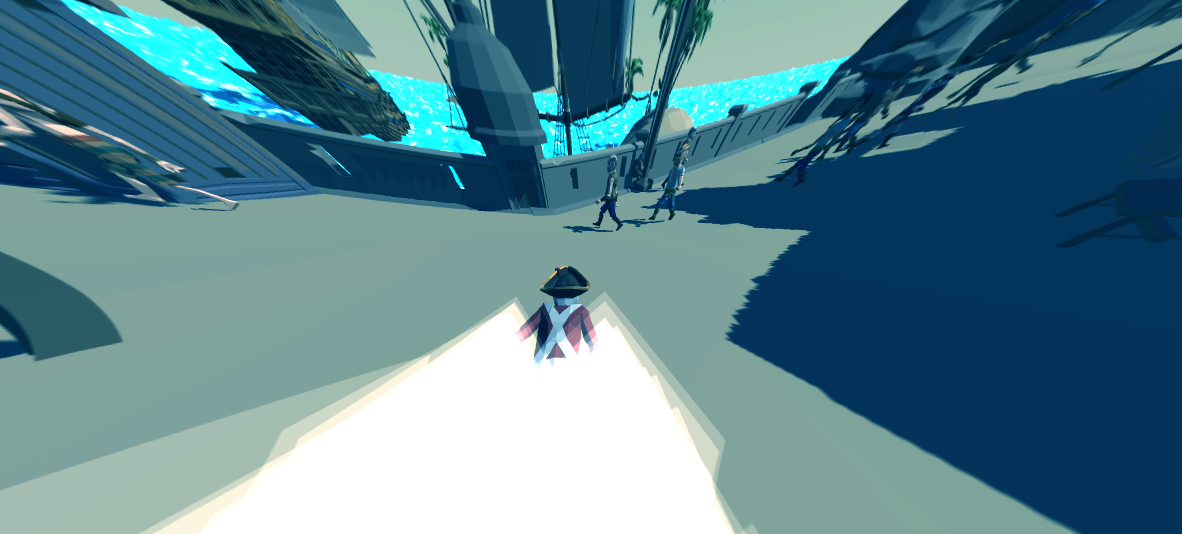
\includegraphics[scale=0.35]{speed.png}
				\caption{Agonie d'un personnage empoisonné}
			\end{figure}
			\FloatBarrier
		
		

